
%(BEGIN_QUESTION)
% Copyright 2006, Tony R. Kuphaldt, released under the Creative Commons Attribution License (v 1.0)
% This means you may do almost anything with this work of mine, so long as you give me proper credit

In any automated (controlled) system, there is a {\it process variable}, a {\it setpoint}, and a {\it manipulated variable}.  There is also something called a {\it load}, which influences how well the control system is able to maintain setpoint.  Provide a general description for a ``load,'' and then identify the load(s) in each of the following manually-controlled processes:

\vskip 30pt
\begin{multicols}{2}
{\bf Example 1:} Temperature control application

$$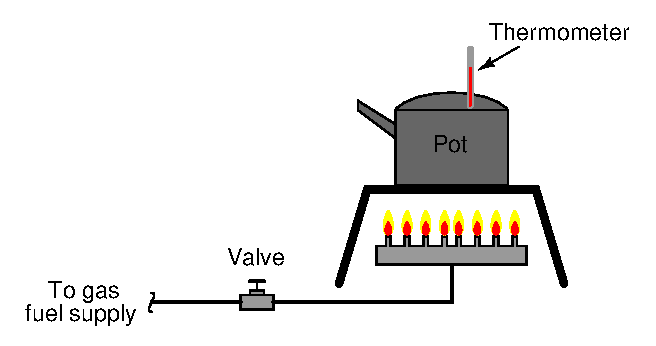
\includegraphics[width=1\columnwidth]{i01453x01.eps}$$

\vskip 30pt

\filbreak
\noindent
{\bf Example 2:} Level control application

$$\includegraphics[width=1\columnwidth]{i01453x02.eps}$$

\vskip 30pt

\filbreak
\noindent
{\bf Example 3:} Flow control application

$$\includegraphics[width=1\columnwidth]{i01453x03.eps}$$

\vskip 30pt

\filbreak
\noindent
{\bf Example 4:} Temperature control application

$$\includegraphics[width=1\columnwidth]{i01453x04.eps}$$
\end{multicols}
\vskip 20pt \vbox{\hrule \hbox{\strut \vrule{} {\bf Suggestions for Socratic discussion} \vrule} \hrule}

\begin{itemize}
\item{} Explain why ambient air temperature is considered a {\it load} to process example \#4, but the insulation thickness on the heat exchanger is not.
\end{itemize}

\underbar{file i01453}
\vfil \eject
%(END_QUESTION)





%(BEGIN_ANSWER)

A {\it load} is any variable in a process (besides the manipulated variable) that has influence over the process variable being controlled.

\vskip 10pt

Note: the following answers are not exhaustive.  In other words, there may be more loads than what is listed here for each process!

\begin{itemize}
\item{} Example 1: ambient air temperature
\item{} Example 2: incoming flow rate
\item{} Example 3: upstream and downstream pressures
\item{} Example 4: steam flow rate, steam temperature
\end{itemize}

%(END_ANSWER)





%(BEGIN_NOTES)

Students may be tempted to list process {\it constants} (such as vessel volume, heat exchanger tube thickness, etc.) as loads because they do impact the process dynamics.  However, the term ``load'' is typically reserved for some {\it variable} that has impact over the process, and is thus liable to change over time in such a way to challenge the loop controller.

To put this in different terms, the need to change setpoints, and the existence of variable loads in a process, both {\it justify} the presence of a controller.  If we were faced with a process never needing a different setpoint, and devoid of variable loads, there would be no need to place a control loop in it!  We could simply set a manually-actuated control valve where we wanted it to be, and leave it in that position forever!

\vfil \eject

\noindent
{\bf Prep Quiz:}

The definition of a {\it load} with regard to process control loops is:

\begin{itemize}
\item{} The time lag between a change in output and a change seen in the PV
\vskip 5pt 
\item{} The value at which the control system attempts to stabilize the PV over time
\vskip 5pt 
\item{} A device that dissipates energy in a circuit, as opposed to sourcing energy to the circuit
\vskip 5pt 
\item{} The multiplication factor of a process, measured from output to input
\vskip 5pt 
\item{} A drain of energy on a system, causing it to operate inefficiently
\vskip 5pt 
\item{} A variable affecting the PV, that is itself unregulated by the control system
\end{itemize}



%INDEX% Control, basics: load (definition)

%(END_NOTES)


